\classheader{10-06-2017}


\section*{The Order Topology}

Given an ordered set $X$ with a binary relation $<$ such that for all $x,y,z\in X$ with $x\neq y$, we have that

\begin{enumerate}
	\item $x\not < x$
	\item $x < y$ or $y<x$
	\item If $x<y$ and $y<z$, then $x<z$
	
	
\end{enumerate}

\definition{The \textbf{order topology} on $X$ is defined to be the topology generated by the base of all open intervals. That is, if $a<b$, then $\left\{  x | a<x<b   \right\}$ is a base element.}

We'll observe that in $\R$, this is the standard topology.

\definition{If $X$ is an ordered set and $Y=\prod\limits_1^n X_i$ is a finite product of copies of $X$, then $Y$ inherits an ordering called the \textbf{dictionary} or \textbf{lexicographic order}, where $(x_1,x_2,x_3,\dots,x_n) < (y_1,y_2,y_3,\dots,y_n)$ if and only if $x_i=y_i$ in the first $k-1$ positions and $x_k<y_k$.}

In $\R^2$ with the order topology, open sets looks like open vertical strips with two open rays adjoined


\begin{figure}[!htb]
	\centering
	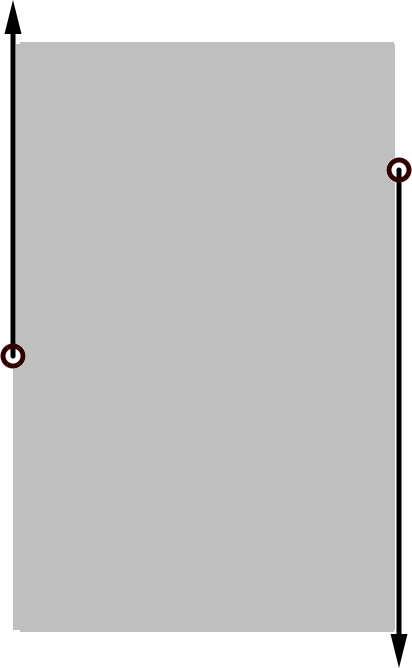
\includegraphics[scale=.2]{images/ordertopr2}
	\caption{An example of an open interval in the order topology on $\R^2$}
	\label{fig:ordtopr2}
\end{figure}

\section*{Convergence in Uncountable Product Spaces}

On $\R^I$, the set of functions $I\rightarrow \R$, we have three topologies: the product, the uniform, and the box topologies.  We also have that while the uniform topology is metrizable (clearly, as it comes from a metric), the box and product topologies are not.

Given a sequence $\left\{f_i\right\}\subset \mathbb{R}^I$:

The sequence $\left\{f_i\right\}$ converges in the product topology if and only if it converges pointwise.

The sequence $\left\{f_i\right\}$ converges in the uniform topology if and only if it converges uniformly, in the analytic sense.  That is, given $\epsilon>0$, there exists an $n\in\mathbb{N}$ such that for all $i>n$, $|f_i(x)-f(x)|< \epsilon$ everywhere.

The sequence $\left\{f_i\right\}$ converges in the box topology if and only if it converges pointwise and there exists an $n\in \mathbb{N}$ such that for all $i>n$, $f_i$ is constant everywhere except a finite set.


\thrm{(Weierstrass) If $\left\{f_i\right\}$ is a sequence of continuous functions which converges to a function $f$ in the uniform topology, then the limit $f$ is also a continuous function.}

\begin{proof}
	
	Take $x,y\in I$, and look at $|f(x)-f(y)|$.  Let $\epsilon>0$ be given.  By the triangle inequality, $|f(x)-f(y)| \leq |f_i(x)-f(x)| + |f_i(x)-f_i(y)|+|f_i(y)-f(y)|$.  By uniform convergence, there exists an $n\in\mathbb{N}$ such that $|f_i(x) - f(x)|$ and $|f_i(y)-f(y)|$ are each less than $\frac{\epsilon}{3}$.  Since each $f_i$ is continuous, there exists a $\delta >0$ such that $|x-y| < \delta$ implies $|f_n(x)-f_n(y)|<\frac{\epsilon}{3}$.  
	
	Thus, whenever $|x-y|<\delta$, we have that $|f(x)-f(y)| \leq |f_n(x)-f(x)| + |f_n(x)-f_n(y)|+|f_n(y)-f(y)| \leq \frac{\epsilon}{3} +\frac{\epsilon}{3} +\frac{\epsilon}{3} = \epsilon$, hence $f$ is continuous.
	
	\end{proof}
	
	
	
\definition{A topological space is \textbf{connected} if it cannot be written as the union of two (non-empty) disjoint open sets.}

\definition{A topological space is \textbf{disconnected} if there exist open sets $A,B$ such that $X=A\cup B$ and $A\cap B=\emptyset$.}



\thrm{A topological space $X$ is connected if and only if $\emptyset$ and $X$ are the only sets which are both closed and open in $X$.}

\begin{proof}
	
	If there exists some non-empty set $K$ which is both open and closed, the the complement of $K$ is also both closed and open, so $X=K\cup X-K$ is a way to write $X$ as the union of two disjoint open sets.  Thus $X$ is connected if and only if the only such $K$ is $X$ itself.
	
	
	\end{proof}


\definition{A \textbf{connected component} of a topological space $X$ is a set which is both closed and open in $X$.}

A topological space can be decomposed into connected components.

\thrm{Let $\sim$ denote the relation $x\sim y$ if and only if there is a connected open set $U$ containing $x$ and $y$.  Then $\sim$ is a proper equivalence relation and the set $\left\{ x | x\sim y \right\}$ is an equivalent characterization of the connected component of $y$.}

\corollary{If the above equivalence relation partitions $X$ into exactly one class, $X$ is connected.}

\definition{A topological space $X$ is \textbf{path connected} if for all $x,y\in X$ there exists a continuous function $p:[0,1]\rightarrow X$ such that $p(0)=x$ and $p(1)=y$.}

We can do a similar thing as above to describe path connected components with an equivalence relation.


	